\section{Evaluation}
\label{sec:evaluation}

\subsection{Experimental Setup}
\label{subsec:setup}

All experiments serve Llama-3.1-8B-Instruct~\cite{dubey2024llama3} in FP16 through vLLM on a single
NVIDIA A100 GPU (40GB). Each scheduling policy is evaluated at seven request
arrival rates (5, 10, 20, 30, 40, 50, and 60 requests/second) on each dataset,
with requests drawn from the dataset in a fixed, pre-computed admission order
per policy and submitted to vLLM's offline generation API as described in
Section~\ref{sec:implementation}.

\subsection{Datasets}
\label{subsec:datasets}

We use two 1{,}000-request evaluation subsets constructed from the public
LMSYS-Chat-1M conversation dataset~\cite{zheng2023lmsyschat,lmsys2024website}. Dataset~1 is a
uniform in-distribution sample used to measure baseline scheduling behavior.
Dataset~2 deliberately over-samples from the extremes of the true
output-length distribution to induce distribution shift between the
predictor's training data and its evaluation data, matching the
out-of-distribution stress test used to evaluate the original LTR
predictor~\cite{fu2024efficient}. Both subsets are reconstructed from the
public dataset release rather than the original framework's unpublished
23{,}800-sample training file, and results should be read as evaluated on a
reconstructed split rather than an exact reproduction.

\subsection{Scheduling Policies and Metrics}
\label{subsec:policies-metrics}

The four scheduling policies compared are summarized in
Table~\ref{tab:scheduling_policies}. We report: (i) mean throughput in
tokens/second; (ii) two indicators of HOL blocking, the ratio of p90 to mean
per-token latency at high load and the slope of mean latency against request
rate, where a flatter, lower-ratio curve indicates less blocking; (iii)
time-to-first-token (TTFT), measuring the delay between request arrival and
the first generated token, which is directly sensitive to queuing delay
independent of a request's total output length; (iv) peak GPU memory
allocation and utilization; and (v) Kendall's tau~\cite{kendall1938new} between each score and true
output length, measuring ranking quality independent of the absolute
scheduling outcome.

\subsection{Throughput}
\label{subsec:results-throughput}

Table~\ref{tab:throughput} reports mean throughput for each scheduler.
LTR + Prompt Length achieves the highest throughput of the four policies on
both datasets, improving over the original LTR scheduler by approximately
31.7\% on Dataset~1 and 6.7\% on Dataset~2. Notably, the original LTR and
Classification schedulers both under-perform plain FCFS on Dataset~1 despite
their explicit goal of reducing HOL blocking, which suggests that a
miscalibrated or overly aggressive reordering can trade away throughput even
as it changes tail-latency behavior; the composite score's use of prompt
length as a stabilizing signal appears to avoid this failure mode on the
datasets tested.
\input{tables/throughput}

\subsection{Latency Versus Request Rate}
\label{subsec:results-latency}

Figure~\ref{fig:latency-vs-rate} shows mean per-token latency as request rate
increases from 5 to 60 requests/second. All four policies show latency
rising with request rate, as expected once the arrival rate approaches the
GPU's sustainable throughput, but the rate of increase differs by policy;
Table~\ref{tab:hol_blocking} quantifies this rate as the latency-vs-rate
slope, discussed in Section~\ref{subsec:results-hol}.

\subsection{Time-to-First-Token}
\label{subsec:results-ttft}

Figure~\ref{fig:ttft-vs-rate} reports mean and p90 TTFT across the same
request-rate sweep. At the highest tested rate (60 requests/second), mean
TTFT for LTR + Prompt Length is 0.157s, compared with 1.034s for FCFS, 0.594s
for Classification, and 0.600s for the original LTR scheduler; the
corresponding p90 TTFT is 0.288s for LTR + Prompt Length versus 1.825s for
FCFS. Because TTFT measures queuing delay directly rather than being
normalized by a request's eventual output length, this gap is a more direct
indication of reduced HOL blocking under the composite scheduler than the
per-token latency metrics in Section~\ref{subsec:results-latency} alone.
\begin{figure}[H]
    \centering

    \begin{subfigure}{\linewidth}
        \centering
        \includegraphics[width=\linewidth]{figures/latency_dataset1.png}
        \caption{Dataset 1 (in-distribution)}
        \label{fig:latency-d1}
    \end{subfigure}

    \vspace{2mm}

    \begin{subfigure}{\linewidth}
        \centering
        \includegraphics[width=\linewidth]{figures/latency_dataset2.png}
        \caption{Dataset 2 (out-of-distribution)}
        \label{fig:latency-d2}
    \end{subfigure}

    \caption{Mean per-token latency versus request rate, by scheduler.}
    \label{fig:latency-vs-rate}
\end{figure}
\begin{figure*}[t]
    \centering
    \begin{subfigure}[b]{0.48\textwidth}
        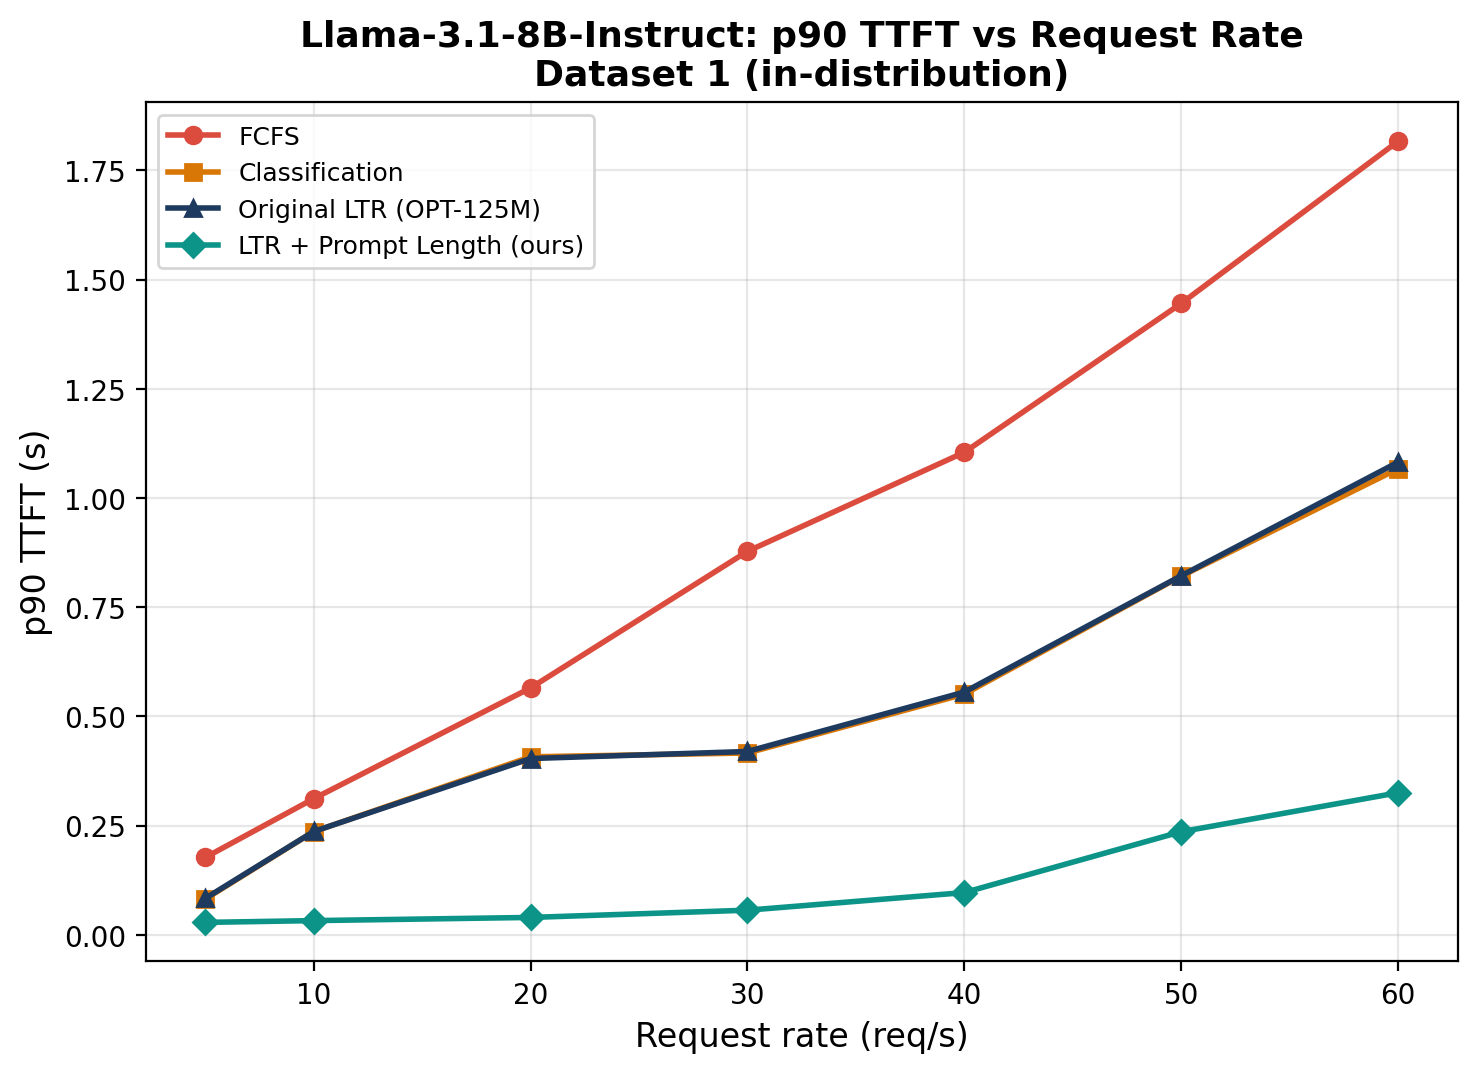
\includegraphics[width=\linewidth]{figures/ttft_p90_dataset1.png}
        \caption{Dataset 1 (in-distribution)}
        \label{fig:ttft-d1}
    \end{subfigure}
    \hfill
    \begin{subfigure}[b]{0.48\textwidth}
        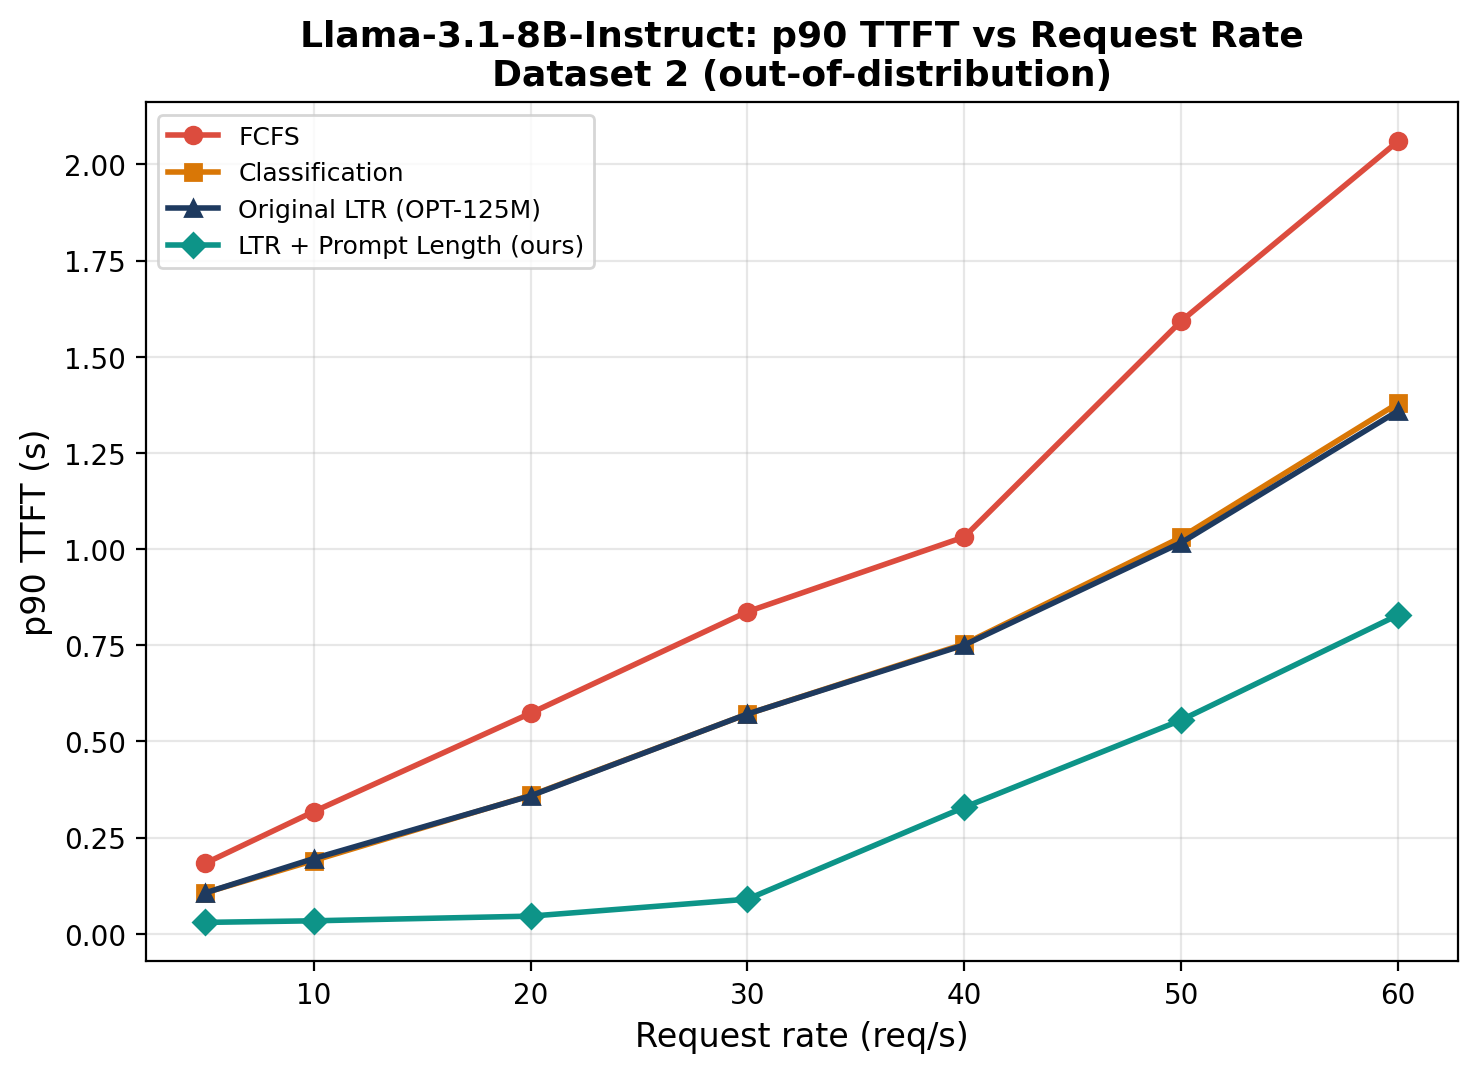
\includegraphics[width=\linewidth]{figures/ttft_p90_dataset2.png}
        \caption{Dataset 2 (out-of-distribution)}
        \label{fig:ttft-d2}
    \end{subfigure}
    \begin{subfigure}[b]{0.48\textwidth}
        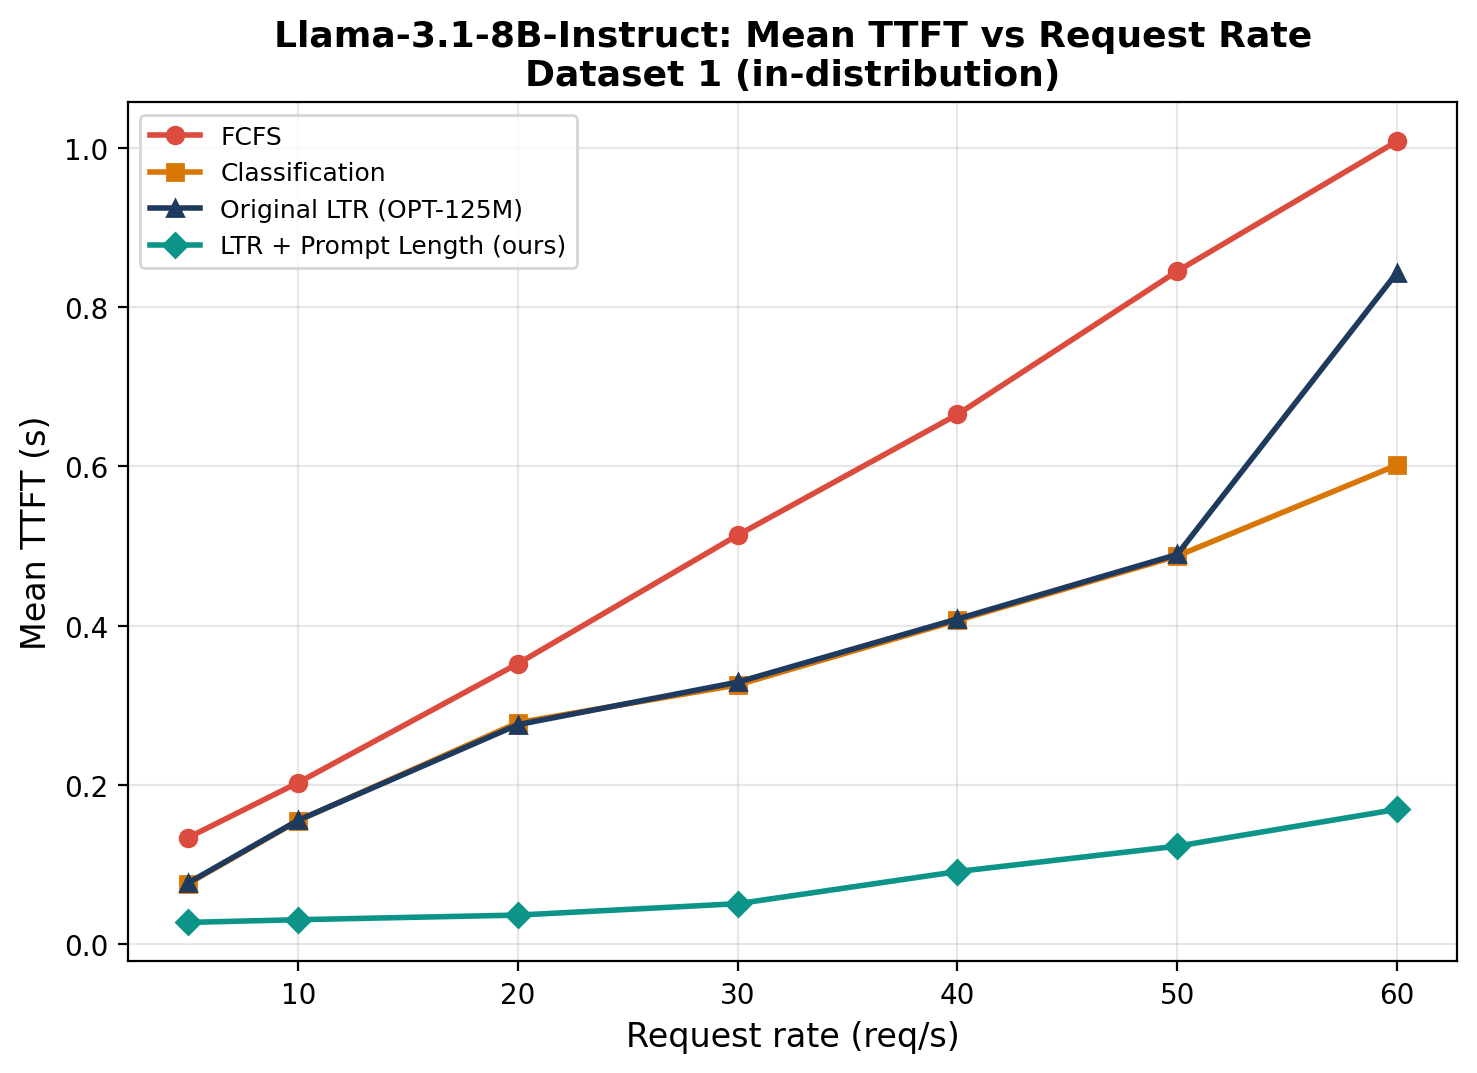
\includegraphics[width=\linewidth]{figures/ttft_mean_dataset1.png}
        \caption{Dataset 1 (in-distribution)}
        \label{fig:ttft-d1}
    \end{subfigure}
    \hfill
    \begin{subfigure}[b]{0.48\textwidth}
        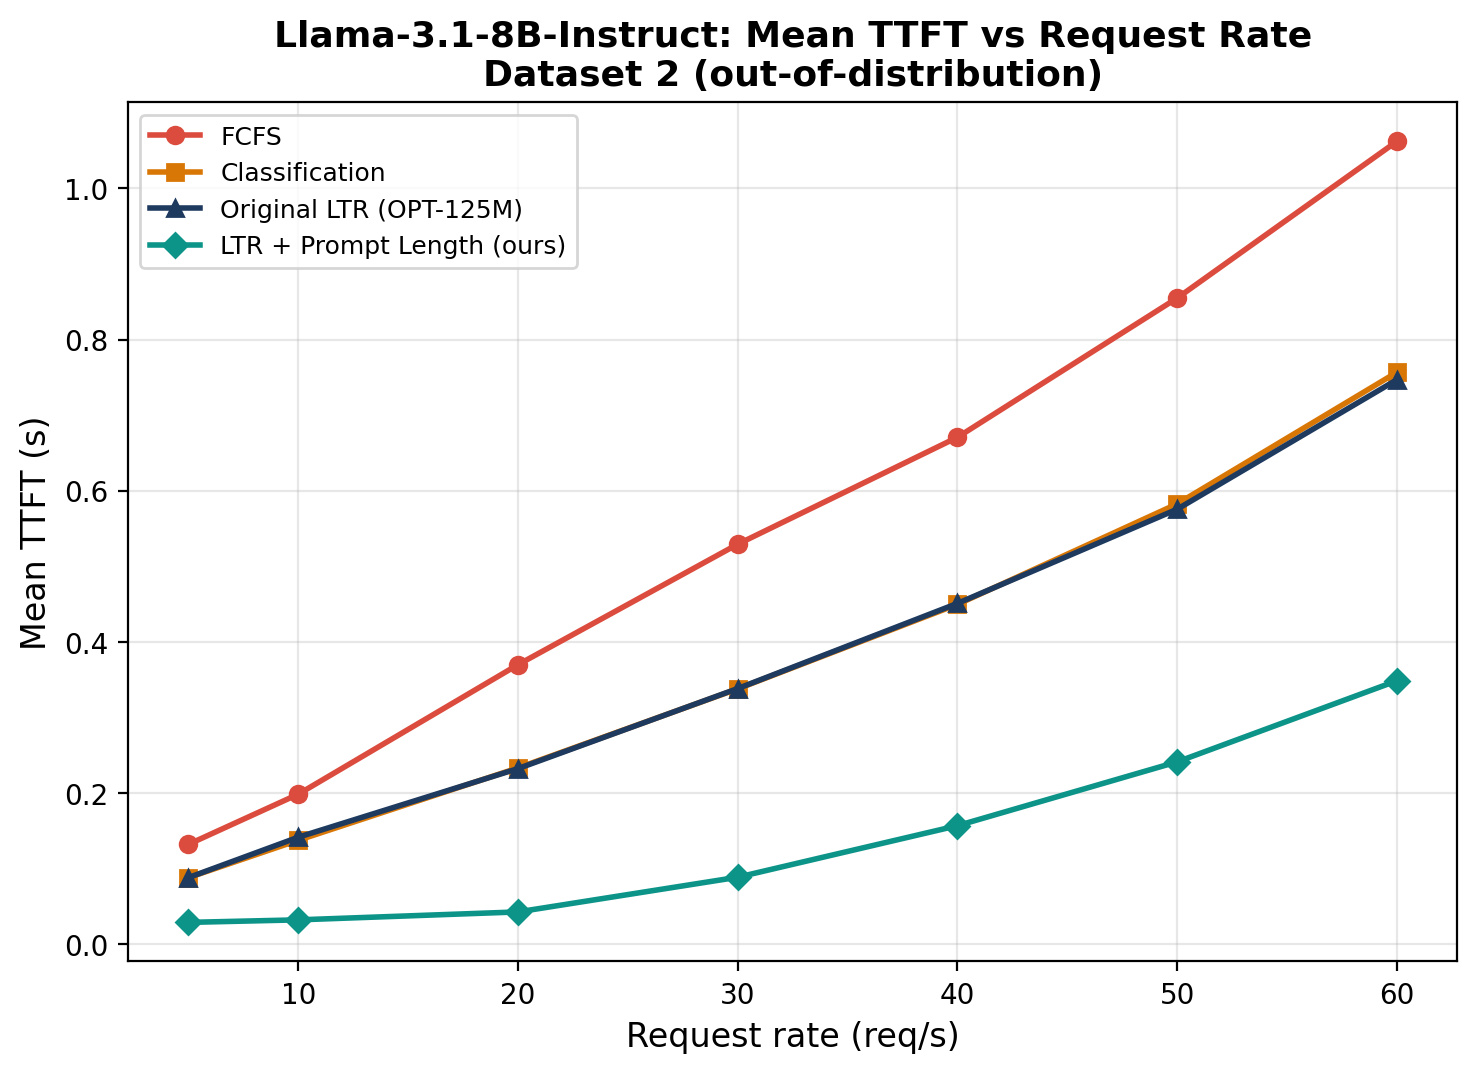
\includegraphics[width=\linewidth]{figures/ttft_mean_dataset2.png}
        \caption{Dataset 2 (out-of-distribution)}
        \label{fig:ttft-d2}
    \end{subfigure}
    \caption{Mean and p90 time-to-first-token versus request rate, by
    scheduler.}
    \label{fig:ttft-vs-rate}
\end{figure*}

\input{tables/hol_blocking}
\input{tables/hol_blocking}
\input{tables/gpu_utilization}
\input{tables/kendalls_tau}

\subsection{Head-of-Line Blocking Indicators}
\label{subsec:results-hol}

Table~\ref{tab:hol_blocking} and Figure~\ref{fig:hol-blocking} summarize the
p90/mean latency ratio at high load and the latency-vs-rate slope for each
scheduler. The Classification and original LTR schedulers achieve the lowest
p90/mean ratio on Dataset~1, indicating that when their length estimate is
accurate, they compress tail latency effectively; however, both show a
steeper latency-vs-rate slope than FCFS on Dataset~1, meaning their latency
degrades faster as load increases. LTR + Prompt Length achieves the lowest
latency-vs-rate slope on Dataset~2 (the out-of-distribution set) among all
four policies, consistent with the intuition that the prompt-length signal
provides a stabilizing effect precisely when the learned predictor is
operating outside its training distribution. Notably, LTR + Prompt Length's p90/mean ratio on Dataset 2 is nonetheless the highest of the four schedulers, indicating that its tail latency still grows in proportion to its mean under distribution shift even as that growth compounds more slowly across increasing request rates than it does for the other three policies. FCFS's slope on Dataset 1 is the flattest of the four despite its poor tail-latency ratio, underscoring that these two indicators capture distinct aspects of HOL blocking rather than a single underlying quantity.

\begin{figure}[H]
    \centering

    \begin{subfigure}{\linewidth}
        \centering
        \includegraphics[width=\linewidth]{figures/hol_blocking_ratio.png}
        \caption{p90/mean latency ratio at high load}
        \label{fig:hol-ratio}
    \end{subfigure}

    \vspace{2mm}

    \begin{subfigure}{\linewidth}
        \centering
        \includegraphics[width=\linewidth]{figures/hol_blocking_slope.png}
        \caption{Latency-vs-request-rate slope}
        \label{fig:hol-slope}
    \end{subfigure}

    \caption{HOL blocking indicators by scheduler and dataset.}
    \label{fig:hol-blocking}
\end{figure}
\subsection{GPU Resource Utilization}
\label{subsec:results-gpu}

Table~\ref{tab:gpu_utilization} and Figure~\ref{fig:gpu-utilization} report
peak GPU memory allocation and utilization measured while serving each
dataset. Memory utilization remains above 86\% of the profiled budget on both
datasets, indicating that the composite scheduler's reordering step does not
introduce additional memory overhead relative to the serving engine's
baseline footprint; the reordering computation itself operates on tokenized
prompt lengths and predictor scores, both of which are negligible in memory
compared to the model weights and KV cache.



\subsection{Ranking Quality: Kendall's Tau}
\label{subsec:results-tau}

Table~\ref{tab:kendalls_tau} reports Kendall's tau between each score and the
true output length on the Dataset~2 (out-of-distribution) held-out set. The
composite score achieves a small improvement over the LTR-only score
(0.3445 to 0.3457, $\Delta = +0.0011$), indicating that the prompt-length
signal does not degrade ranking quality under distribution shift and offers a
modest, consistent improvement even independent of its effect on the
scheduling-level metrics reported above.
\begin{figure}[H]
    \centering
    \includegraphics[width=0.85\linewidth,height=5.2cm,keepaspectratio]{figures/gpu_utilization.png}
    \caption{Peak GPU memory allocation, peak reserved memory, and memory
    utilization by dataset.}
    \label{fig:gpu-utilization}
\end{figure}
\subsection{Throughput by Scheduler, Averaged Across Request Rates}
\label{subsec:results-throughput-avg}

Figure~\ref{fig:throughput-avg} presents the same throughput comparison as
Table~\ref{tab:throughput} averaged across all seven tested request rates
rather than aggregated once per dataset, confirming that the ordering in
Table~\ref{tab:throughput} is not an artifact of any single request rate.

\begin{figure}[H]
    \centering
    \includegraphics[width=0.85\linewidth,height=5.0cm,keepaspectratio]{figures/throughput_by_scheduler.png}
    \caption{Mean throughput by scheduler, averaged across all tested
    request rates.}
    \label{fig:throughput-avg}
\end{figure}
